\subsection{Design}
\paragraph{Nutzerinteraktion}
Für die Art der Benutzerinteraktion des Programms sind mehrere Ansätze denkbar.
Beispielsweise könnte das Programm mit jeweils verschiedenen, aufeinanderfolgenden
Befehlen von der Kommandozeile aus aufgerufen werden wie in Abb. \ref{simple-gui-example}
dargestellt. Alternativ könnte das Program, wie in Abb. \ref{graphical-gui-example} skizziert,
mit einer kompletten, grafischen Oberfläche versehen werden.

\paragraph{}
Als pragmatischer, einfacher und funktionaler Ansatz wurde ein Mittelweg gewählt
bei dem eine Konsolenanwendung beim Start alle einzelnen konfigurierten
Zielwerte auf jeweils einer Zeile darstellt, geöffnet bleibt und auf Tasteneingaben
wartet um entweder eine seiner Funktionen auszuführen oder beendet zu werden (siehe Abb. \ref{post-start}
im Kapitel \ref{Kundendokumentation} - Kundendokumentation).


\begin{figure}
    \caption{Nutzerinteraktion mit aufeinanderfolgenden Befehlen}
    \label{simple-gui-example}
    \begin{minted}[bgcolor=codebg]{bash}
        >_ terminal-config-manager show
    
        1 Anwendung a mit Wert -> b
        2 Anwendung c mit Wert -> d
    
        >_ terminal-config-manager change 2
    
        1 Anwendung a mit Wert -> b
        2 Anwendung c mit Wert -> e
    \end{minted}
\end{figure}

\begin{figure}
    \caption{Nutzerinteraktion über eine grafische Oberfläche und Buttons, skizzenhaft}
    \label{graphical-gui-example}
    \centering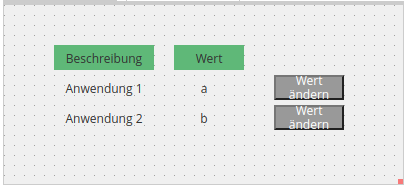
\includegraphics[scale=0.6]{gui-example.png}
\end{figure}

\paragraph{Softwaredesign}
Jeweils funktional zusammengehörige Teile des Quellcodes wurden so gut wie möglich
von anderen Teilen separiert. Die hauptsächliche Organisationsebene bilden dabei
Module, die sich in jeweils einer Quellcodedatei befinden. Beispielsweise ist dadurch
Programmcode, der mit der Verarbeitung von Tasteneingaben betraut ist, im Modul

\begin{minted}[bgcolor=codebg]{bash}
    src/UserInterface/Input.hs
\end{minted}

lokalisiert. Programmcode, welcher mit dem Dateisystem interagiert, dagegen
hier:

\begin{minted}[bgcolor=codebg]{bash}
    src/Infrastructure/FileModification.hs
\end{minted}

Den einzelnen Modulen übergeordnet befindet sich eine Organisationsebene, welche
versucht einem möglichen Ansatz aus dem Kontext des Domain-Driven-Design \cite{domain-driven-design} gerecht
zu werden. Dabei werden Teile des Programmcode in verschiedene Gruppen organisiert,
beispielsweise \textbf{Application}, \textbf{Domain}, \textbf{Infrastructure} und \textbf{Userinterface}, und es wird
darauf geachtet, dass Abhängigkeiten zwischen Modulen dieser Gruppen stets in
eine bestimmte Richtung zeigen. Wenn dieses Schema eingehalten wird, dann können
Probleme, wie zyklische Abhängigkeiten oder schlecht erweiterbare Module, reduziert
oder ganz vermieden werden. Das angestrebte Schema ist dem Buch Domain-Driven-Design \cite{domain-driven-design}
entnommen und ist in Abb. \ref{domain-driven-design-layers} im Angang dargestellt.
Zum Vergleich wurden die tatsächlichen Modulabhängigkeiten mit Unterstützung von
Softwaretools \cite{graphmod} \cite{xdot} ausgelesen und in einem Graphen dargestellt.
In Kapitel \ref{domain-driven-design-result} - Ergebnisdiskussion wird ein Vergleich
angestellt.